%\documentclass[smaller,handout]{beamer}
%\documentclass[smaller,handout]{beamer}
\def\bmode{0} % Mode 0 for presentation, mode 1 for a handout with notes, mode 2 fo% r handout without notes
\if 0\bmode
\documentclass[smaller]{beamer}
\else \if 1\bmode
\immediate\write18{pdflatex -jobname=\jobname-Handout-Notes\space\jobname}
\documentclass[smaller,handout]{beamer}
\usepackage{handoutWithNotes}
\pgfpagesuselayout{2 on 1 with notes}[letterpaper, landscape, border shrink=4mm]
\else \if 2\bmode
\immediate\write18{pdflatex -jobname=\jobname-Handout\space\jobname}
\documentclass[smaller,handout]{beamer}
\fi
\fi
\fi

%%%%%%%%%%%%%%%%%%%%%%%%%%%%%%%%%%%%%%%%%%%%%%%%%%%%%%%%%%%%%%%%%%%%%%%%%%%%%%%%%%%%%%%%%%%%%
\newcommand{\coursetitle}{CEE 616: Probabilistic Machine Learning}
\newcommand{\longlecturetitle}{M2 Linear Methods: L2C Linear Regression}
\newcommand{\shortlecturetitle}{L2C: Linear Regression}
\newcommand{\instructor}{Jimi Oke}
\newcommand{\lecturedate}{Thu, Oct 2, 2025}
%%%%%%%%%%%%%%%%%%%%%%%%%%%%%%%%%%%%%%%%%%%%%%%%%%%%%%%%%%%%%%%%%%%%%%%%%%%%%%%%%%%%%%%%%%%%%

 
% \usepackage[T1]{fontenc} 
% \usepackage{lmodern} 
%\usepackage{etex}
 %\newcommand{\num}{6{} }

% \usetheme[
%   outer/progressbar=foot,
%   outer/numbering=fraction,
%   block=fill,
%   inner/subsectionpage=progressbar
% ]{metropolis}
\usetheme{Madrid}
\useoutertheme[subsection=false]{miniframes} % Alternatively: miniframes, infolines, split
\useinnertheme{circles}
% %\useoutertheme{Frankfurt}
% \usecolortheme{beaver}
% %\useoutertheme{crane}
% %\useoutertheme{metropolis}
\usepackage[backend=biber,style=authoryear,maxcitenames=2,maxbibnames=99,safeinputenc,url=false, eprint=false]{biblatex}
%\addbibresource{bib/references.bib}
% \AtEveryCitekey{\iffootnote{{\tiny}\tiny}{\tiny}}

% %\usepackage{pgfpages}
% %\setbeameroption{hide notes} % Only slides
% %\setbeameroption{show only notes} % Only notes
% %\setbeameroption{hide notes} % Only notes
% %\setbeameroption{show notes on second screen=right} % Both

% % \usepackage[sfdefault]{Fira Sans}

% % \setsansfont[BoldFont={Fira Sans}]{Fira Sans Light}
% % \setmonofont{Fira Mono}

% %\usepackage{fira}
% %\setsansfont{Fira}
% %\setmonofont{Fira Mono}
% % To give a presentation with the Skim reader (http://skim-app.sourceforge.net) on OSX so
% % that you see the notes on your laptop and the slides on the projector, do the following:
% % 
% % 1. Generate just the presentation (hide notes) and save to slides.pdf
% % 2. Generate onlt the notes (show only nodes) and save to notes.pdf
% % 3. With Skim open both slides.pdf and notes.pdf
% % 4. Click on slides.pdf to bring it to front.
% % 5. In Skim, under "View -> Presentation Option -> Synhcronized Noted Document"
% %    select notes.pdf.
% % 6. Now as you move around in slides.pdf the notes.pdf file will follow you.
% % 7. Arrange windows so that notes.pdf is in full screen mode on your laptop
% %    and slides.pdf is in presentation mode on the projector.

% % Give a slight yellow tint to the notes page
% \setbeamertemplate{note page}{\pagecolor{yellow!5}\insertnote}\usepackage{palatino}

% %\usetheme{metropolis}
% %\usecolortheme{beaver}
 \usepackage{tipa}
% \usepackage{enumerate}
\definecolor{darkcandyapplered}{HTML}{A40000}
\definecolor{lightcandyapplered}{HTML}{e74c3c}

% %\setbeamercolor{title}{fg=darkcandyapplered}

% \definecolor{UBCblue}{rgb}{0.04706, 0.13725, 0.26667} % UBC Blue (primary)
% \definecolor{UBCgrey}{rgb}{0.3686, 0.5255, 0.6235} % UBC Grey (secondary)

% % \setbeamercolor{palette primary}{bg=darkcandyapplered,fg=white}
% % \setbeamercolor{palette secondary}{bg=darkcandyapplered,fg=white}
% % \setbeamercolor{palette tertiary}{bg=darkcandyapplered,fg=white}
% % \setbeamercolor{palette quaternary}{bg=darkcandyapplered,fg=white}
% % \setbeamercolor{structure}{fg=darkcandyapplered} % itemize, enumerate, etc
% % \setbeamercolor{section in toc}{fg=darkcandyapplered} % TOC sections
% % \setbeamercolor{frametitle}{fg=darkcandyapplered,bg=white} % TOC sections
% % \setbeamercolor{title in head/foot}{bg=white,fg=white} % TOC sections
% % \setbeamercolor{button}{fg=darkcandyapplered} % TOC sections

% % % Override palette coloring with secondary
% % \setbeamercolor{subsection in head/foot}{bg=lightcandyapplered,fg=white}

%\usecolortheme{crane}
% \makeatletter
% \setbeamertemplate{headline}{%
%   \begin{beamercolorbox}[colsep=1.5pt]{upper separation line head}
%   \end{beamercolorbox}
%   \begin{beamercolorbox}{section in head/foot}
%     \vskip1pt\insertsectionnavigationhorizontal{\paperwidth}{}{}\vskip1pt
%   \end{beamercolorbox}%
%   \ifbeamer@theme@subsection%
%     \begin{beamercolorbox}[colsep=1.5pt]{middle separation line head}
%     \end{beamercolorbox}
%     \begin{beamercolorbox}[ht=2.5ex,dp=1.125ex,%
%       leftskip=.3cm,rightskip=.3cm plus1fil]{subsection in head/foot}
%       \usebeamerfont{subsection in head/foot}\insertsubsectionhead
%     \end{beamercolorbox}%
%   \fi%
%   \begin{beamercolorbox}[colsep=1.5pt]{lower separation line head}
%   \end{beamercolorbox}
% }
% \makeatother

% Reduce size of frame box
\setbeamertemplate{frametitle}{%
    \nointerlineskip%
    \begin{beamercolorbox}[wd=\paperwidth,ht=2.0ex,dp=0.6ex]{frametitle}
        \hspace*{1ex}\insertframetitle%
    \end{beamercolorbox}%
}


%\setbeamercolor{frametitle}{bg=darkcandyapplered!80!black!90!white}
%\setbeamertemplate{frametitle}{\bf\insertframetitle}

%\setbeamercolor{footnote mark}{fg=darkcandyapplered}
%\setbeamercolor{footnote}{fg=darkcandyapplered!70}
%\Raggedbottom
%\setbeamerfont{page number in head/foot}{size=\tiny}
%\usepackage[tracking]{microtype}


% %\usepackage[sc,osf]{mathpazo}   % With old-style figures and real smallcaps.
% %\linespread{1.025}              % Palatino leads a little more leading

% % Euler for math and numbers
% %\usepackage[euler-digits,small]{eulervm}
% %\AtBeginDocument{\renewcommand{\hbar}{\hslash}}
\usepackage{graphicx,multirow,booktabs}
\usepackage{animate}
\usepackage{media9}


% %\mode<presentation> { \setbeamercovered{transparent} }

\setbeamertemplate{navigation symbols}{}
\makeatletter
\def\beamerorig@set@color{%
  \pdfliteral{\current@color}%
  \aftergroup\reset@color
}
\def\beamerorig@reset@color{\pdfliteral{\current@color}}
\makeatother


% %=== GRAPHICS PATH ===========
\graphicspath{{./m2-images/}}
% % Marginpar width
% %Marginpar width
% %\setlength{\marginparsep}{.02in}


% %% Captions
% % \usepackage{caption}
% % \captionsetup{
% %   labelsep=quad,
% %   justification=raggedright,
% %   labelfont=sc
% % }

% \setbeamerfont{caption}{size=\footnotesize}
% \setbeamercolor{caption name}{fg=darkcandyapplered}

% %AMS-TeX packages

\usepackage{amssymb,amsmath,amsthm,mathtools} 
\usepackage{bm}
\DeclareMathOperator*{\argmax}{arg\,max}
\DeclareMathOperator*{\argmin}{arg\,min}
% \usepackage{color}

% %https://tex.stackexchange.com/a/31370/2269
\usepackage{mathtools,cancel}

\renewcommand{\CancelColor}{\color{red}} %change cancel color to red

\makeatletter
\let\my@cancelto\cancelto %copy over the original cancelto command
\newcommand<>{\cancelto}[2]{\alt#3{\my@cancelto{#1}{#2}}{\mathrlap{#2}\phantom{\my@cancelto{#1}{#2}}}}
% redefine the cancelto command, using \phantom to assure that the
% result doesn't wiggle up and down with and without the arrow
\makeatother


% %\usepackage{comment}
% %\usepackage{hyperref,enumerate}
% \usepackage{minitoc,array}

% \definecolor{slblue}{rgb}{0,.3,.62}
% % \hypersetup{
% %     colorlinks,%
% %     citecolor=blue,%
% %     filecolor=blue,%
% %     linkcolor=blue,
% %     urlcolor=slblue
% % }

% \usepackage{epstopdf}
% \epstopdfDeclareGraphicsRule{.gif}{png}{.png}{convert gif:#1 png:\OutputFile}
% \AppendGraphicsExtensions{.gif}

% %\usepackage{listings}

% %%% TIKZ
% \usepackage{forest}
\usepackage{tikz}
\usepackage{pgfplots}
\usepackage{pgfplotstable}
%\usepackage{pgfgantt}
\pgfplotsset{compat=newest}

\usetikzlibrary{fit,arrows,shapes,positioning,shapes.geometric}
\usetikzlibrary{decorations.markings}
\usetikzlibrary{shadows,automata}
\usetikzlibrary{patterns}
\usetikzlibrary{trees,mindmap,backgrounds}
%\usetikzlibrary{circuits.ee.IEC}
\usetikzlibrary{decorations.text}
% % For Sagnac Picture
% \usetikzlibrary{%
%     decorations.pathreplacing,%
%     decorations.pathmorphing%
% }
% \tikzset{no shadows/.style={general shadow/.style=}}
% %
% %\usepackage{paralist}

% \tikzset{
%   font=\Large\sffamily\bfseries,
%   red arrow/.style={
%     midway,red,sloped,fill, minimum height=3cm, single arrow, single arrow head extend=.5cm, single arrow head indent=.25cm,xscale=0.3,yscale=0.15,
%     allow upside down
%   },
%   black arrow/.style 2 args={-stealth, shorten >=#1, shorten <=#2},
%   black arrow/.default={1mm}{1mm},
%   tree box/.style={draw, rounded corners, inner sep=1em},
%   node box/.style={white, draw=black, text=black, rectangle, rounded corners},
% }

% %%% FORMAT PYTHON CODE
% %\usepackage{listings}
% % Default fixed font does not support bold face
% \DeclareFixedFont{\ttb}{T1}{txtt}{bx}{n}{8} % for bold
% \DeclareFixedFont{\ttm}{T1}{txtt}{m}{n}{8}  % for normal

% % Custom colors
% \definecolor{deepblue}{rgb}{0,0,0.5}
% \definecolor{deepred}{rgb}{0.6,0,0}
% \definecolor{deepgreen}{rgb}{0,0.5,0}

% %\usepackage{animate}

% % Python style for highlighting
% % \newcommand\pythonstyle{\lstset{
% % language=Python,
% % basicstyle=\footnotesize\ttm,
% % otherkeywords={self},             % Add keywords here
% % keywordstyle=\footnotesize\ttb\color{deepblue},
% % emph={MyClass,__init__},          % Custom highlighting
% % emphstyle=\footnotesize\ttb\color{deepred},    % Custom highlighting style
% % stringstyle=\color{deepgreen},
% % frame=tb,                         % Any extra options here
%     % showstringspaces=false            % 
% % }}

% % % Python environment
% % \lstnewenvironment{python}[1][]
% % {
% % \pythonstyle
% % \lstset{#1}
% % }
% % {}

% % % Python for external files
% % \newcommand\pythonexternal[2][]{{
% % \pythonstyle
% % \lstinputlisting[#1]{#2}}}

% % Python for inline
% % 
% % \newcommand\pythoninline[1]{{\pythonstyle\lstinline!#1!}}

% %\usepackage{algorithm2e}

\newcommand{\eps}{\epsilon}
\newcommand{\bX}{\mb X}
\newcommand{\by}{\mb y}
\newcommand{\bbe}{\bm\beta}
\newcommand{\beps}{\bm\epsilon}
\newcommand{\bY}{\mb Y}

\newcommand{\osn}{\oldstylenums}
\newcommand{\dg}{^{\circ}}
\newcommand{\lt}{\left}
\newcommand{\rt}{\right}
\newcommand{\pt}{\phantom}
\newcommand{\tf}{\therefore}
\newcommand{\?}{\stackrel{?}{=}}
\newcommand{\fr}{\frac}
\newcommand{\dfr}{\dfrac}
\newcommand{\ul}{\underline}
\newcommand{\tn}{\tabularnewline}
\newcommand{\nl}{\newline}
\newcommand\relph[1]{\mathrel{\phantom{#1}}}
\newcommand{\cm}{\checkmark}
\newcommand{\ol}{\overline}
\newcommand{\rd}{\color{red}}
\newcommand{\bl}{\color{blue}}
\newcommand{\pl}{\color{purple}}
\newcommand{\og}{\color{orange!90!black}}
\newcommand{\gr}{\color{green!40!black}}
\newcommand{\dca}{\color{darkcandyapplered}}
\newcommand{\nin}{\noindent}
\newcommand*\circled[1]{\tikz[baseline=(char.base)]{
            \node[shape=circle,draw,thick,inner sep=1pt] (char) {\small #1};}}

\newcommand{\bc}{\begin{compactenum}[\quad--]}
\newcommand{\ec}{\end{compactenum}}

\newcommand{\p}{\partial}
\newcommand{\pd}[2]{\frac{\partial{#1}}{\partial{#2}}}
\newcommand{\dpd}[2]{\dfrac{\partial{#1}}{\partial{#2}}}
\newcommand{\pdd}[2]{\frac{\partial^2{#1}}{\partial{#2}^2}}
\newcommand{\pde}[3]{\frac{\partial^2{#1}}{\partial{#2}\partial{#3}}}
\newcommand{\nmfr}[3]{\Phi\left(\frac{{#1} - {#2}}{#3}\right)}
\newcommand{\Err}{\text{Err}}
\newcommand{\err}{\text{err}}

%\DeclarePairedDelimiter\ceil{\lceil}{\rceil}
%\DeclarePairedDelimiter\floor{\lfloor}{\rfloor}

%%%% GREEK LETTER SHORTCUTS %%%%%
\newcommand{\la}{\lambda}
\renewcommand{\th}{\theta}
\newcommand{\al}{\alpha}
\newcommand{\G}{\Gamma}
\newcommand{\si}{\sigma}
\newcommand{\Si}{\Sigma}


\pgfmathdeclarefunction{poiss}{1}{%
  \pgfmathparse{(#1^x)*exp(-#1)/(x!)}%
  }

\pgfmathdeclarefunction{gauss}{2}{%
  \pgfmathparse{1/(#2*sqrt(2*pi))*exp(-((x-#1)^2)/(2*#2^2))}%
}

\pgfmathdeclarefunction{expo}{2}{%
  \pgfmathparse{#1*exp(-#1*#2)}%
}

\pgfmathdeclarefunction{expocdf}{2}{%
  \pgfmathparse{1 -exp(-#1*#2)}%
}

\newcommand{\mb}{\mathbb}
\newcommand{\mc}{\mathcal}
\newcommand{\tr}{^{\top}}
\newcommand{\pe}{\pause}
% \usepackage{pst-plot}

% \usepackage{pstricks-add}
% \usepackage{auto-pst-pdf}   

% \psset{unit = 3}

% \def\target(#1,#2){%
%  {\psset{fillstyle = solid}
%   \rput(#1,#2){%
%     \pscircle[fillcolor = white](0.7,0.7){0.7}
%     \pscircle[fillcolor = blue!60](0.7,0.7){0.5}
%     \pscircle[fillcolor = white](0.7,0.7){0.3}
%     \pscircle[fillcolor = red!80](0.7,0.7){0.1}}}}
% \def\dots[#1](#2,#3){%
%     \psRandom[
%       dotsize = 2pt,
%       randomPoints = 25
%     ](!#2 #1 0.04 sub sub #3 #1 0.04 sub sub)%
%      (!#2 #1 0.04 sub add #3 #1 0.04 sub add)%
%      {\pscircle[linestyle = none](#2,#3){#1}}}


%%%%%%%%%%%%%%%%%%%%%%%%%%%%%%%%%%%%%%%%%%%%%%%%%%%
%%%%%%%%%%%%%%%%%%%%%%%%%%%%%%%%%%%%%%%%%%%%%%%%%%%
\title[\shortlecturetitle]{ {\normalsize \coursetitle}
  \\ \longlecturetitle}
\date[\lecturedate]{\footnotesize \lecturedate}
\author{{\bf \instructor}}
\institute[UMass Amherst]{
%\titlegraphic{\hfill
  \begin{tikzpicture}[baseline=(current bounding box.center)]
    \node[anchor=base] at (-7,0) (its) {\includegraphics[scale=.3]{UMassEngineering_vert}} ;
  \end{tikzpicture}
  % \hfill\includegraphics[height=1.5cm]{logo}
}

%https://tex.stackexchange.com/questions/55806/mindmap-tikzpicture-in-beamer-reveal-step-by-step
  \tikzset{
    invisible/.style={opacity=0},
    visible on/.style={alt={#1{}{invisible}}},
    alt/.code args={<#1>#2#3}{%
      \alt<#1>{\pgfkeysalso{#2}}{\pgfkeysalso{#3}} % \pgfkeysalso doesn't change the path
    },
  }


% https://tex.stackexchange.com/questions/446468/labels-with-arrows-for-an-equation
% https://tex.stackexchange.com/a/402466/121799
\newcommand{\tikzmark}[3][]{
\ifmmode
\tikz[remember picture,baseline=(#2.base)] \node [inner sep=0pt,#1](#2) {$#3$};
\else
\tikz[remember picture,baseline=(#2.base)] \node [inner sep=0pt,#1](#2) {#3};
\fi
}

% \lstset{language=matlab,
%                 basicstyle=\scriptsize\ttfamily,
%                 keywordstyle=\color{blue}\ttfamily,
%                 stringstyle=\color{blue}\ttfamily,
%                 commentstyle=\color{gray}\ttfamily,
%                 morecomment=[l][\color{gray}]{\#}
%               }


              
\begin{document}

\maketitle

\begin{frame}
  \frametitle{Outline}
  \tableofcontents
\end{frame}




 \section{Introduction}

 \begin{frame}
   \frametitle{Linear regression}
   \pe
   Model of the form:
   \pe
   \begin{equation}
     p(y|\bm x; \bm \th) = \mathcal{N}(y | \bm w\tr\bm x, \sigma^{2})
     \pe =     \fr{1}{\sqrt{2\pi\sigma^{2}}}\exp\lt(-\fr{1}{2\sigma^{2} }(y  - \bm w\tr\bm x)^{2}\rt)
   \end{equation}\pe
   where: \pe
   
   \begin{itemize}
   \item $y$: response or dependent variable
   \item $\bm\th = \bm w$: model parameters\pe
   \item $\bm w = [w_{0}, w_{1},\ldots , w_{D}]$\pe
   \item $w_{0}$: intercept, offset, bias, unconditional mean or baseline $\mb{E}[y]$ \pe
   \item $w_{1:D}$: weights or regression coefficients\pe
     \item $\bm x = [1, x_{1}, \ldots, x_{D}]$: predictors or explanatory/independent variables\pe
   \item $D$: number of features
   \end{itemize}
 \end{frame}

 \begin{frame}
   \frametitle{Complexity}
   \pe
   \begin{itemize}
   \item Simple linear regression: $D=1$: \pe
     \begin{equation}
       p(y|\bm x; \bm \th)  =  \mathcal{N}(y |  w_{0} + w_{1}x, \sigma^{2})
     \end{equation}
     \pe
   \item Multiple linear regression: $D >1$: \pe
     \begin{equation}
     p(y|\bm x; \bm \th) = \mathcal{N}(y | \bm w\tr\bm x, \sigma^{2})
     \end{equation}
     \pe
   \item Multivariate linear regression: $\bm y \in \mb R^{J}, J > 1$
     \pe
     \begin{equation}
       p(\bm y|\bm x; \bm \th) = \prod_{j=1}^{J}\mathcal{N}(y | \bm w\tr\bm x, \sigma^{2})
     \end{equation}
     \pe
   \item LR with nonlinear transformation of inputs: \pe
     \begin{equation}
       p(y|\bm x; \bm \th) = \mathcal{N}(y | \bm w\tr \bm\phi(\bm x), \sigma^{2})
     \end{equation}
     \pe where $\bm\phi(\bm x)$ is feature extractor or kernel
     \pe
     \item Polynomial regression (1D): \pe $\bm\phi(x) = [1, x, x^{2}, \ldots , x^{d}]$ \pe (order/degree $d$)
   \end{itemize}
 \end{frame}

 
 \begin{frame}
  \frametitle{Alternative view of simple linear regression model}
  \pause

  For any fixed value of the independent variable $x$, the dependent variable $y$ is related to $x$ via the \textbf{model equation}:\pause

  \begin{equation}
    \label{eq:50}
    \tikzmark[blue]{T}{y = w_0 + w_1x} + \tikzmark[red]{R}{\bm{\epsilon}}
  \end{equation}
  \pause



    \begin{tikzpicture}[overlay, remember picture,node distance =1.5cm,
    every node/.append style={text width=3cm,align=center},
    shorten >=3pt]
    \node[draw, rectangle, blue] (Tdescr) [below left=of T]{true regression line};
    \draw[blue,->] (Tdescr) to [in=-90,out=90] (T.south);
    \node[draw, rectangle, red] (Rdescr) [below right =of R]{random error term};
    \draw[red,->] (Rdescr) to [in=-90,out=90] (R.south);
  \end{tikzpicture}

  
  \pause

  \vspace{5ex}
  where $\bm\epsilon$ is a normally distributed random variable:

  \pause    
  %\vspace{20ex}
  \begin{equation}
    \label{eq:51}
    \bm\epsilon \sim \mathcal{N}(0, \sigma^2)
  \end{equation}

  \pause

  $w_0$ (intercept) and $w_1$ (slope) are the \textbf{regression coefficients}
\end{frame}

\begin{frame}
  \frametitle{Alternate view 1D LR (cont.)}
  \pause

  Further considerations:\pause

  \begin{itemize}[<+->]
  \item The linear regression model: $y$ is treated as a \textbf{random variable} whose mean depends on $x$
   \begin{align*}
   \begin{split}
   y &= w_0+w_1x+\epsilon\\
   \mbox{[Response]}&=\mbox{[mean (depending on $x$)]}+\mbox{[error]}
   \end{split}
   \end{align*}
   \item $\mb E(y|x)=w_0+w_1x$
   \item Given data $x_n,\ n=1,...,N$, $x$ is \textbf{treated as fixed}.
   \item $\epsilon$ - \textbf{error term} (\textbf{random variable}), accounts for:
   	\begin{itemize}
	\item measurement error of $y$
	\item the effects of other variables not in the model
	\end{itemize}
  \end{itemize}
\end{frame}
\begin{frame}
  \frametitle{Model in matrix notation}
  
  \begin{itemize}
    % \setlength{\itemindent}{-1em}
  \item With $n$ independent observations on $Y$ and the associated values of $x_n$, the complete model:\pause
    %\small
    \begin{align*}
      \begin{split}
        y_1 &= w_0+w_1x_1+\epsilon_1\\
        y_2 &= w_0+w_1x_2+\epsilon_2\\
        &\mathrel{\makebox[\widthof{=}]{\vdots}} \\
        y_N &= w_0+w_1x_N+\epsilon_N
      \end{split}
    \end{align*}
    \normalsize

    \pause
  \item In matrix notation:
    %\scriptsize
    \begin{align*}
      \begin{split}
        \begin{bmatrix}
          {y_1}\\
          y_2\\
          \vdots\\
          y_n
        \end{bmatrix} &= \begin{bmatrix}
          1 & x_1 \\
          1 & x_2 \\
          \vdots & \vdots \\
          1 & x_n
        \end{bmatrix}  \begin{bmatrix}
          w_0\\
          w_1
        \end{bmatrix}+\begin{bmatrix}
          {\epsilon_1}\\
          \epsilon_2\\
          \vdots\\
          \epsilon_n
        \end{bmatrix}\\
        \bm y &=\bm X \bm w + \bm\epsilon
      \end{split}
    \end{align*}

    \item We typically assume an intercept (represented by column of 1's in $\bm X$), except where explicitly noted otherwise.
  \end{itemize}

\end{frame}

\begin{frame}
  \frametitle{Residual sum of squares (RSS)}
  \pause
  \begin{block}{Residual}\pause
    Given $n$ independent observations $(x_1,y_1) ... (x_n, y_n)$, with $\hat y_n$ as the predicted value for each $y_n$, \pause
    the residual $e_n$ is defined as:\pause
    \begin{equation}
      \label{eq:16}
      e_n = y_n - \hat y_n
    \end{equation}
  \end{block}
  \pause
  
  The RSS is an overall measure of the fitness of a regression model: \pause

  \begin{equation}
    RSS = \pause e_1^2 + e_2^2 + \cdots + e_n^2 = \sum_{i=1}^N e_n^2 \pause =  \sum_{i=1}^N \lt(y_{n}- \hat y_{n} \rt)^2
  \end{equation}
  \pause
  \vspace{-2ex}
  \begin{minipage}{.65\linewidth}
    \begin{figure}[h!]
      \centering
      \includegraphics[width=.45\textwidth]{3-2a} \pause
      \includegraphics[width=.45\textwidth]{3-2b}
    \end{figure}
  \end{minipage}\pause
  \begin{minipage}{.3\linewidth}
    \bl  \small $RSS$ plotted against $w_0$ and $w_1$ for a given dataset using a contour plot (Left) and 3-D plot
    (right). The least squares estimate $(\hat w_0,\hat w_1)$ is indicated by the red dots.
  \end{minipage}
\end{frame}

\begin{frame}
  \frametitle{Coefficient of determination}

  The \textbf{total sum of squares} is a measure of the total variance in the data.\\ \pause
    \begin{equation}
      \label{eq:7}
      TSS = \sum_{n=1}^N \lt(y_n - \ol y_n\rt)^2 = \sum_{n=1}^N y_n^2 - \fr1 N \lt(\sum_{n=1}^N y_n\rt)^2
    \end{equation}    

  The coefficient of determination $R^2$ is a measure of the \textbf{\rd proportion of variance explained} by the regression model: \pause
  
  \begin{equation}
    \label{eq:6}
    R^2 = \fr{TSS - RSS}{TSS} = 1 - \fr{RSS}{TSS}
  \end{equation}

  \pe The \textbf{adjusted} $R^{2}$ penalizes for model complexity: \pe
  \begin{equation}
    R^{2}_{a} = 1 - \fr{RSS/df_{RSS}}{TSS/df_{TSS}} \pe = 1 - \fr{(1-R^{2})(N-1)}{N-D-1}
  \end{equation}
\end{frame}

\section{OLS}
\begin{frame}
  \frametitle{Principle of least squares}\pause

  Given the regression model:\pause
  \begin{equation}
    \hat{y}_{n}  = \bm w\tr \bm x_{n}
  \end{equation}
  \pause
  then the residual sum of squares (loss function) is given by \pause
  \begin{eqnarray}
    RSS(\bm w) &=& \sum_{n=1}^{N}(y_{n} - \hat{y}_{n})^{2} \pause = \sum_{n=1}^{N}\lt(y_{n} - \bm w\tr\bm x_{n} \rt)
  \end{eqnarray}
  \pause
  In matrix form, we write:\pause
  \begin{equation}
    RSS(\bm w) = (\bm y - \bm X{\bm w})\tr(\bm y - \bm X{\bm w})
  \end{equation}
  \pause
  To minimize the RSS, we take the derivative w.r.t. to ${\bm w}$ and set to 0:
  \begin{eqnarray*}
    RSS &=& \bm y\tr\bm y - (\bm X{\bm w})\tr\bm y - \bm y\tr(\bm X{\bm w}) + (\bm X{\bm w})\tr\bm X{\bm w} \\\pause
        &=& \bm y\tr\bm y - 2(\bm X{\bm w})\tr\bm y + {\bm w}\tr\bm X\tr\bm X {\bm w} \\\pause
    RSS' &=& -2\bm X\tr\bm y + 2\bm X\tr\bm X{\bm w} \pause = -2\bm X\tr(\bm y - \bm X{\bm w})% \\\pause
  %  \implies \bm X\tr(\bm y - \bm X {\bm w}) &=& 0
  \end{eqnarray*}
\end{frame}

\begin{frame}
  \frametitle{Principle of least squares (cont.)}\pause
  
  If $\bm X_{N\times D+1}$ has full column rank (i.e. all columns are linearly independent), then:\pause

  \begin{itemize}
  \item $\bm X\tr\bm X$ is positive definite
  \item $\bm X\tr\bm X$ is nonsingular and therefore invertible
  \end{itemize}
  This means there is a unique solution to the normal equations:
  \pause
  \begin{eqnarray}
    \bm X\tr(\bm y - \bm X\bm w)   &=& 0 \\\pause
    (\bm X\tr\bm X)\bm w           &=& \bm X\tr\bm y \\\pause
    \hat{\bm w}                       &=& (\bm X\tr\bm X)^{-1}\bm X\tr\bm y 
  \end{eqnarray}

  \pause

  We therefore obtain the predictions as:\pause
  \begin{equation}
    \hat{\bm y} = \bm X\hat{\bm w} = \bm X (\bm X\tr\bm X)^{-1}\bm X\tr\bm y 
  \end{equation}
\end{frame}




\begin{frame}
  \frametitle{Ordinary least squares (OLS) model}
  \pause

     \begin{equation}
      \underset{(N \times 1)}{\bm y} = \underset{(N\times (D+1)}{\bm X} \cdot \underset{((D+1)\times 1)}{\bm {\bm w}} +
       \underset{(N \times 1)}{\bm\epsilon}
    \end{equation}
    \pause
    where the least squares estimator can be written compactly in matrix form as:\pause
    \begin{equation}
      \bm{\hat{\bm w}}_{OLS} = (\bm{X}\tr\bm{X})^{-1}\bm{X}\tr{\bm y}
    \end{equation}
    \pause
    $\bm{\hat{\bm w}}$ is unbiased: \pause $\mb{E}(\bm{\hat{\bm w}}) = \bm{\hat{\bm w}}$.
   \pause

  The error terms are assumed to satisfy:\pause
  \begin{itemize}
  \item \textbf{Zero mean:} \pause $\mb{E}(\bm\epsilon) = \bm 0$\pe
  \item \textbf{Constant variance:} \pause $Cov(\bm\epsilon) = \sigma^2 \bm I$
  \end{itemize}

  \pause

  The regression line passes through the centroid of the data points $(\ol x, \ol y)$
\end{frame}

\begin{frame}
  \frametitle{Obtaining predictions}
  \pe
  Once we have the OLS estimate, $\hat{\bm w}_{OLS}$, we can predict a set of  responses $\hat{\bm y}$ from  observations $\bm X$ using: \pe
  \begin{eqnarray}
    \hat{\bm y} &=& \bm X\hat{\bm w}_{OLS} \pe \\\pe
                &=& {\pl \bm X   (\bm{X}\tr\bm{X})^{-1}\bm{X}\tr}{\bm y}\\\pe
    &=& {\pl \bm X^{\dagger}} \bm y
  \end{eqnarray}
  \pe
  \begin{itemize}
  \item ${\pl \bm X^{\dagger}=  \bm X   (\bm{X}\tr\bm{X})^{-1}\bm{X}\tr}$ is known as the \textbf{hat matrix} or \textbf{projection matrix} or left pseudo-inverse of $\bm X$\pe
  \end{itemize}
\end{frame}
\begin{frame}
  \frametitle{OLS assumptions}
  The ordinary least squares estimate for regression coefficients gives  the {\bl\it B}est {\bl\it L}inear {\bl\it U}nbiased {\bl\it E}stimate
  ({\bl BLUE}): \textbf{Gauss-Markov theorem}.

  \medskip
  
  \pe 
  Assumes the following conditions are met:
\pe
\begin{description}[labelwidth=\widthof{Homsc}]
  \item[Linearity:] the parameters we are estimating using the OLS  method must be themselves linear.
  \item[Randomness:] our data must have been randomly sampled from the population.
  \item[NoN-Collinearity:] the regressors being calculated are not perfectly correlated with each other.
  \item[Exogeneity:] the regressors are not correlated with the error term.
  \item[Homoscedasticity:] no matter what the values of our regressors might be, the error of the variance is constant.
  \end{description}
\end{frame}

 
 \section{Considerations}


%\subsection{2.1 Qualitative predictors}
\begin{frame}
  \frametitle{Qualitative predictors}
  \pause

  \begin{itemize}[<+->]
  \item Qualitative predictors arise when the \textit{levels} are categories, e.g.
    \begin{itemize}[<+->]
    \item gender
    \item income levels
    \item commuting mode
    \item type of soil
    \item climate zone
    \end{itemize}
  \item These predictors are referred to as \textit{factors}
  \end{itemize}
\end{frame}

\begin{frame}
  \frametitle{Representing qualitative predictors: two-level case}
  \pause

   
    A factor with two possible values is represented by an \textbf{indicator} (or \textbf{dummy}) variable.\\ \pause

    \bigskip
    
    For instance, if $X$ is a factor denoting married status, then:\pause
    \begin{equation*}
      x_{n} =      \begin{cases}
        0 & \text{if $i$th person is unmarried}\\
        1 & \text{if $i$th person is married}
      \end{cases}
    \end{equation*}
    \pause
    Then in the simple case, the linear model would be:\pause
    \begin{equation*}
      y_n = w_0 + w_1x_n + \epsilon_n =
       \begin{cases}
        w_0 + \eps_n & \text{if $i$th person is unmarried}\\
       w_0 + w_1 + \epsilon_n & \text{if $i$th person is married}
      \end{cases}
    \end{equation*}
    \pause
    An alternative to the $\{0/1\}$ scheme is $\{-1/1\}$.
\end{frame}

\begin{frame}
  \frametitle{Representing qualitative predictors: multi-level case}
  \pause

  When more than two levels exist, additional dummy variables may be used. \\ \pause

  \bigskip

  Generally, $k-1$ dummy variables are used to represent $k$ levels. \pause 
  \begin{align*}
    x_{nB} &=
    \begin{cases}
      0 & \notin B\\
      1 & \in B
    \end{cases}\\ \pause
    x_{nC} &=
    \begin{cases}
      0 & \notin C\\
      1 & \in C
    \end{cases}\\ \pause
    y_n &= w_0 + w_Bx_{nB} + w_Cx_{nC} =
          \begin{cases}
            w_0 + \epsilon_n           &  \notin{B\cup C} \\
            w_0 + w_B + \epsilon_n &  \in{B} \\
            w_0 + w_C + \epsilon_n &  \in{C} 
          \end{cases}
  \end{align*}
  \pause
  The level with no dummy variable is termed the \textbf{baseline}. \pause If $A = \ol{B\cup C}$, then $A$ is the baseline.
\end{frame}

%\subsection{2.2 Interaction terms}
\begin{frame}
  \frametitle{Interaction terms}\pause
  We introduce interaction terms into a linear model if \textit{synergistic} effects are observed between two variables, i.e.\ the effect of one variable depends on the value of the other. \pause

  \bigskip

  For instance, if $x_1$ and $x_2$ interact in the standard model:\pause
  \begin{equation}
    Y = w_0 + w_1x_{1} + w_2x_2 + \epsilon
  \end{equation}
  \pause
  then, we include the \textbf{interaction term} $x_1x_2$:\pause
  \begin{equation}
    Y = w_0 + w_1x_1 + w_2x_2 + w_3x_1x_2 + \epsilon
  \end{equation}
  In models with interaction terms, the \textbf{main effects} must be included by keeping the single variables.
\end{frame}

% \begin{frame}
%   \frametitle{Activity 2: Estimate and interpret models with dummy variables and
%     interaction terms}
%   \pause

%   The \texttt{\bl Carseats} dataset contains 400 simulated observations of child car seats from different stores.\pause

%   \begin{itemize}[<+->]
%   \item Create a linear fit using all the variables along with the interaction terms: \texttt{Income:Advertising} and \texttt{Price:Age}
%   \item Interpret the coefficients of the interaction terms (use the \texttt{contrasts()} function to view the coding scheme for the dummy variables)
%   \item Verify the signs of all the coefficients make sense
%   \item Identify which predictors (including interaction terms) you would drop
%   \item Use the $F$-test to further support your decision(s)
%   \end{itemize}
  
% \end{frame}


%\subsection{Higher order terms}
\begin{frame}
  \frametitle{Polynomial regression}\pause
  In some cases, a polynomial function provides a good approximation to the true regression function for a given dataset. \pause

  \begin{center}
    \visible<3->{\includegraphics[width=0.4\textwidth]{polyfit1}}
    \visible<4->{\includegraphics[width=0.4\textwidth]{polyfit2}}
  \end{center}
 
  \pause

   \begin{block}{$d$-th degree polynomial regression model equation}\pause
    \begin{equation}
      \label{eq:20}
      y =  w_0 + w_1 x + w_2 x^2 + \cdots + w_d x^d+ \epsilon
    \end{equation}
    \pause
    where $\bm\epsilon$ is normally distributed: \pause $\mathcal{N}(0, \sigma^2)$
  \end{block}

  \pause

  This means that the expected value of $y$ given $x$ can be written as:\pause
  \begin{equation}
    \label{eq:21}
    \mb{E}(y|x) = w_0 + w_1 x + w_2 x^2 + \cdots + w_d x^d
  \end{equation}
 \end{frame}



\begin{frame}
  \frametitle{Polynomial regression and multiple regression}
  Polynomial regression can be considered a special case of multiple linear regression.\\ \pause

  For example, consider the model:
  \begin{equation*}
    Y = w_0 + w_1x + w_2 x^2 + \bm\epsilon
  \end{equation*}

  \pause

  If we set $x \to z_1$ and $x^2 \to z_2$, then the model becomes:\pause

  \begin{equation*}
    Y = w_0 + w_1z_1 + w_2z_2 +\bm\epsilon
  \end{equation*}
  \pause

  which can be taken as a multiple linear regression model with two predictor variables.
\end{frame}

\begin{frame}
  \frametitle{Improving model quality via higher-order terms}
  \pause

  The presence of nonlinearity in the ``residuals vs.\ fitted'' plot usually indicates the form of the required polynomial.
  \pause

  \begin{exampleblock}{Example 2.1: \texttt{mpg} $\sim$ \texttt{weight}}
    In the \texttt{Auto} dataset, we regress \texttt{\bl mpg} on \texttt{\bl weight}. \pause

    \begin{figure}[h!]
      \centering
      \includegraphics[width=.4\textwidth]{autolm1}
      \caption{Simple linear model: $y = w_0 + w_1x$. $R^2 = 0.69$. Is this a good fit?}
    \end{figure}
  \end{exampleblock}
\end{frame}

\begin{frame}
  \frametitle{Improving model quality via higher-order terms (cont.)}
  \pause
 

  \begin{exampleblock}{Example 2.1: \texttt{mpg} $\sim$ \texttt{weight} (cont.)}
    We observe a pattern in the residual plot against the fitted values.\pause
    
    \begin{figure}[h!]
      \centering
      \visible<3->{\includegraphics[width=.4\textwidth]{autolm1res}}
      \caption{``Residuals vs. fitted values'' plot for the simple linear model. What do you observe?}
    \end{figure}

    \pause

    \vspace{-2ex}
    This further confirms that a linear fit is not the best approximation for this data.
  \end{exampleblock}
\end{frame}

\begin{frame}
  \frametitle{Improving model quality via higher-order terms (cont.)}
  \pause
 

  \begin{exampleblock}{Example 2.1: \texttt{mpg} $\sim$ \texttt{weight} (cont.)}

    \pause

    Now, we try the model: \pause $Y = w_0 + w_1X + w_2X^2$.\pause
    \begin{figure}[h!]
      \centering
      \visible<4->{\includegraphics[width=.4\textwidth]{autolm2}}
      \caption{Linear and quadratic models for regressing \texttt{\bl mpg} on \texttt{\bl weight}.}
    \end{figure}

    \pause

    The adjusted $R^2$ is now 0.71.
  \end{exampleblock}
\end{frame}

\begin{frame}
    \frametitle{Improving model quality via higher-order terms (cont.)}

    \pause

  \begin{exampleblock}{Example 2.1: \texttt{mpg} $\sim$ \texttt{weight} (cont.)}

    \pause

    We compare the residual plots.
    
    \begin{figure}[h!]
      \centering
      \visible<3->{\includegraphics[width=.4\textwidth]{nonlinear}}
      \caption{Residual plots for the linear and quadratic models for regressing \texttt{\bl mpg} on \texttt{\bl weight}.}
    \end{figure}

    \pause

    \vspace{-3ex}

    While we have explained some of the variance with the second-order term, the statistics reveal that other variables may also be important predictors.
  \end{exampleblock}
    
\end{frame}

\section{Irregularities}
\begin{frame}
  \frametitle{When OLS assumptions fail}
  \pause

  In some cases, assumptions for the ordinary least squares may not hold due a combination of the following.
  \bigskip
  
  \pause

  
  \begin{alertblock}{Data issues encountered in linear regression}
  \begin{enumerate}[<+->]
  \item Nonlinearity
  \item Correlation of error terms 
  \item Non-constant variance of error  (heteroscedasticity)
  \item Outliers
  \item High-leverage points
  \item Collinearity
  \end{enumerate}
\end{alertblock}
  \pause

  We discuss a few approaches to handle these.
\end{frame}

%\subsection{ Nonlinearity}
\begin{frame}
  \frametitle{Nonlinearity}

  \pause

  There are situations in which we can tell from investigations that the predictors do not exhibit a linear relationship with the response variable.\\ \pause

  \bigskip
  
  To handle these, we consider \textbf{linearly transforming} the data (either the inputs or outputs or both.)\\ \pause

  \begin{exampleblock}{Useful intrinsically linear functions}\pause
  \begin{enumerate}[<+->]
  \item $y = \alpha e^{{\bm w} x} \pause  \quad          \alert{\xrightarrow{y' = \ln(y)}}              \pause \quad  y' = \ln(\alpha) + {\bm w} x$ \\
  \item $y = \alpha x^{{\bm w}}   \pause  \quad          \alert{\xrightarrow{y' = \ln(y),\, x' = \ln(x)}} \pause \quad  y' = \ln(\alpha) + {\bm w} x'$\\
  \item $y = \alpha + {\bm w}\cdot \log(x) \pause\quad  \alert{\xrightarrow{x'=\log(x)}}               \pause \quad  y = \alpha + {\bm w} x'$\\
  \item $y = \alpha + {\bm w}\cdot \fr1x \pause  \quad  \alert{\xrightarrow{x'= \fr1x}}                \pause \quad  y = \alpha + {\bm w} x'$
  \end{enumerate}
  \end{exampleblock}
\end{frame}

% \begin{frame}
%   \frametitle{Using a log transformation}\pause
%   In the Boston housing price dataset, we observe a nonlinear relationship between \texttt{medv} and \texttt{lstat}.\pause

%   \begin{figure}[h!]
%     \centering
%     \includegraphics[width=.4\textwidth]{logtrans1}
%     \includegraphics[width=.4\textwidth]{logtrans2}
%     \caption{Log transformation of \texttt{lstat} in Boston housing price dataset}
%   \end{figure}

%   \pause
  
%   The log transformation partially addresses this issue. You can check the impact on $R^2$.
% \end{frame}

%\subsection{3.2 Correlation of error terms}
\begin{frame}
  \frametitle{Autocorrelation}
  Correlation of error terms can lead to underestimation of coefficient standard errors: \pause
  $Cov(\epsilon_n,\epsilon_k) \ne 0 \quad \forall\quad n\ne k, k = 1,...,n$
  \pause
  \begin{itemize}[<+->]
  \item Identified by patterns in residual trends
  \item This usually occurs in time series or geographical data
  \end{itemize}
  \pause

 
  \begin{figure}[h!]
    \centering
    \includegraphics[width=.42\textwidth]{autocor-ex}
    \caption{Example of error correlations for a time series dataset. The blue dashed lines represent the 95\% confidence interval. Correlations outside of this band are statistically significant.}
  \end{figure}
\end{frame}

% \begin{frame}
%   \frametitle{Autocorrelation (cont.)}\pause
%   In the \texttt{hpdata.lm2} model, there are a few problematic observations (why?), although the average is close to 0.
%   \pause
%   \begin{figure}[h!]
%     \centering
%     \visible<3->{\includegraphics[width=.52\textwidth]{autocor2}}
%     \caption{Autocorrelation plot for housing data model including all variables}
%   \end{figure}
%   \pause
%   \vspace{-3ex}
%   This can be addressed by specifying a different error structure.
% \end{frame}

%\subsection{3.3 NoN-constant variance}
\begin{frame}
  \frametitle{Non-constant variance of error terms}
  \pause

  Recall a fundamental assumption of linear regression is \textbf{\rd homoscedasticity}, i.e. \pause
  \begin{equation}
    \label{eq:20}
    Var(\eps_n) = \sigma^2
  \end{equation}

  \pause

  
  \begin{figure}[h!]
    \centering
    \visible<4->{\includegraphics[width=.8\textwidth]{3-11}}
    \caption{Heteroscedasticity (left) and homoscedasticity (right); fixed by log-transformation of the response.}
  \end{figure}
  
\end{frame}

%\subsection{Outliers}
\begin{frame}
  \frametitle{Outliers}
  \pause

  \begin{itemize}[<+->]
  \item Outliers occur when some observations produce residuals that are significantly larger than average
  \item They can be efficiently identified using \textbf{studentized residuals}:
    \begin{equation}
      t_n = \fr{\hat e_n}{RSE\sqrt{1-h_{n}}}
    \end{equation}
  \item To address this issue, outliers can be \textbf{carefully} removed from the training data
  \end{itemize}
  \pause

  \begin{figure}[h!]
    \centering
    \visible<5->{\includegraphics[width=.8\textwidth]{3-12}}
    \caption{Outlier in a regression model. The studentized residual confirms the outlier cannot be ignored.}
  \end{figure}
\end{frame}


%\subsection{3.5 High leverage}
\begin{frame}
  \frametitle{High leverage points}
  \pause

  \begin{block}{Leverage}
    The leverage of an observation is a measure of its influence on the regression model:\pause
  \begin{equation}
    \label{eq:21}
    h_n = \fr1n + \fr{(x_n - \ol x)^2}{\sum_{k=1}^N(x_k -\ol x)^2}
  \end{equation}
\end{block}
\pause

  \begin{itemize}[<+->]
  \item Leverage increases with the deviation from the mean
  \item Leverage is often plotted against the standardized residuals to identify problematic observations
  \item Another quantity, the Cook's distance, explicitly computes the scaled average of the changes to regression model when the observation of interest is removed
  \item $\fr1n \le h_n \le 1$; $\mb{E}(h_n) = \fr{p+1}{n}$
  \end{itemize}
\end{frame}

% \begin{frame}[fragile]
%   \frametitle{Leverage: identification}\pause
%   Recall the model: \texttt{hpdata.lm2}, the leverage plot is shown below.
%   \pause
%   \begin{figure}[h!]
%     \centering
%     \visible<3->{\includegraphics[width=.5\textwidth]{leverage}}
%     \caption{Standardized residuals plotted against leverage for a multivariate linear model. Which observations have a high leverage?}
%     \label{fig:lev}
%   \end{figure}
  
% \end{frame}


%\subsection{3.6 Collinearity}
\begin{frame}
  \frametitle{Collinearity}

  \pause

  Collinearity arises when two or more predictors are correlated. \pause This can usually be identified via correlation plots:
\pause
  \begin{figure}[h!]
    \centering
    \visible<4->{\includegraphics[width=.5\textwidth]{corr}}
    \caption{Correlation plot for a few of the predictors in the \texttt{Credit} dataset. Which of the predictors in this plot are highly correlated?}
    \label{fig:cor}
  \end{figure}
  
\end{frame}

\begin{frame}
  \frametitle{Identifying collinearity}\pause
  \textbf{\rd Consequences}\pause 
  \begin{itemize}[<+->]
  \item Increases uncertainty of model estimates (standard errors)
  \item Reduces the power of the hypothesis test (probability of correctly rejecting the null hypothesis)
  \end{itemize}

  \pause

  How do we \textbf{\gr identify} collinearity?\pause

  \begin{itemize}[<+->]
  \item Identify using correlation plots and values
  \item Use the variance inflation factor (VIF), which is robust to \textit{multicollinearity}:\pause
    \begin{equation}
      \label{eq:24}
      VIF(\hat w_j) = \fr{1}{1 - R^2_{X_j|X_{-j}}}
    \end{equation}\pause
    where $R^2_{X_j|X_{-j}}$ is the $R^2$ from a regression of $X_j$ onto all of the other predictors.

    \item Variables with similarly high VIFs are multicollinear.
    \item The smallest value of the VIF is 1.
  \end{itemize}
  
\end{frame}

\begin{frame}[fragile]
  \frametitle{Correcting for collinearity}
  \pause

  To correct for [multi]collinearity, there are two approaches:\pause
  \begin{itemize}[<+->]
  \item Remove the problematic variables (e.g.\ if 3 variables are multicollinear, drop 2 of them from the model )
  \item Create a composite variable from the collinear variables
  \end{itemize}
  \pause

  \begin{exampleblock}{Example: Regressing Balance on Income, Limit, Rating and Age (\texttt{Credit} dataset) }\pause
    For example, if we estimate the model:
    \begin{equation*}
      Y = w_0 + w_1X_1 + w_2X_2 + w_3X_3 + w_4X_4
    \end{equation*}
    \pause where $Y, X_1, X_2, X_3$ are \texttt{Balance}, \texttt{Income}, \texttt{Limit}, \texttt{Rating} and \texttt{Age}, respectively. \pause
    The adjusted $R^2$ is 0.876 and the VIF values are: \pause
    \vspace{-1ex}{\bl\scriptsize
\begin{verbatim}
       Income:    2.52
       Limit:     149
       Rating:    149
       Age:       1.03
\end{verbatim}}
  \end{exampleblock}

\end{frame}


\begin{frame}[fragile]
  \frametitle{Correcting for collinearity (cont.)}
  \begin{exampleblock}{Example: Regressing Balance on Income, Limit, Rating and Age (\texttt{Credit} dataset); cont. }\pause
    We see from the VIF that Limit and Age are highly correlated. \pause
    So we remove \texttt{\bl Limit} ($X_2$) and estimate the new model:
    \begin{equation*}
      Y = w_0 + w_1X_1 + w_3X_3 + w_4X_4
    \end{equation*}
    \pause
    The adjusted $R^2$ is only slightly lower at 0.875, and the VIFs are:    \pause
    \vspace{-2ex}{\bl
\begin{verbatim}
      Income:    2.52
      Rating:    2.48
      Age:       1.02
\end{verbatim}    }
      \pause
      Thus, we have corrected for collinearity without decreasing the quality of the fit.
  \end{exampleblock}
\end{frame}

% \begin{frame}[fragile]
%   \frametitle{Correcting for collinearity (cont.)}
%   \begin{exampleblock}{Example: Regressing \texttt{Balance} on \texttt{Income}, \texttt{Limit}, \texttt{Rating} and \texttt{Age} (\texttt{Credit} dataset); cont. }\pause
%     Finally, we remove \texttt{\bl Age} ($X_4$), as it has a high p-value and hence an unreliable predictor
%     \begin{equation*}
%       Y = w_0 + w_1X_1 + w_3X_3
%     \end{equation*}
%     \pause
%     The adjusted $R^2$ in this final case remains 0.875.     
%   \end{exampleblock}
% \end{frame} 


\section{WLS}
\begin{frame}
  \frametitle{Weighted least squares (WLS)}
  \pe
  When variances are not heteroskedastic (i.e. they are not constant), then we use the WLS model: \pe
  \begin{equation}
    p(y|\bm x;\bm\th) = \mathcal{N}(y|\bm w\tr\bm x, \sigma^{2}(\bm x ) \pe =
    \fr{1}{\sqrt{2\pi\sigma^{2}(\bm x)}}\exp\lt(-\fr{1}{2\sigma^{2}(\bm x) }(y  - \bm w\tr\bm x)^{2}\rt)
  \end{equation}
  \pe
  Thus, we can write the WLS model for the entire dataset as:\pe
  \begin{equation}
    p(\bm y|\bm x;\bm \th) =\mc{N}(\bm y|\bm X\bm w,\bm\Lambda^{-1})
  \end{equation}
  \pe
  where $\bm\Lambda = \text{diag}(1/\sigma^{2}(\bm x_{n}))$ is a diagonal weight matrix.
  \pe
  \begin{itemize}
  \item In OLS, we assume $\epsilon_{n} \sim \mc{N}(0,\sigma^{2})$ [constant variance]\pe
  \item In WLS, we assume $\epsilon_{n} \sim \mc{N}(0,\sigma^{2}(x_{n})^{2})$ [non-constant variance; different for each observation]
  \end{itemize}
  
\end{frame}

\begin{frame}
  \frametitle{WLS (cont.)}\pe
  The WLS estimator (coefficients) is given by: \pe
  \begin{equation}
    \hat{\bm w}_{WLS} = (\bm X\tr\bm\Lambda\bm X)^{-1}\bm X^{T}\bm\Lambda \bm y
  \end{equation}
  \pe
  \begin{itemize}
  \item Since $\bm\Lambda = \text{diag}(1/\sigma^{2}(\bm x_{n})) = \text{diag}(w_{1},\ldots, w_{N})$ is a diagonal weight matrix, we can write $\bm\Lambda = \bm W$. \pe
  \item Thus, the WLS estimate can be written as:\pe
    \begin{equation}
      \hat{\bm w}_{WLS} = (\bm X\tr\bm W \bm X)^{-1}\bm X^{T}\bm W \bm y
    \end{equation}
    \pe
  \item When $\bm W$ is not known, some common estimators are: $w_{n}  = \fr{1}{x_{n}}$ or $w_{n} = n$
  \item Weights can also be iteratively estimated
  \end{itemize}
\end{frame}


\section{Outlook}

\begin{frame}
  \frametitle{Reading assignments}

  \begin{itemize}
  \item \textbf{PMLI} 11.1-2
  \item \textbf{ESL}   3.2
   \item \textbf{PMLCE} 8.1
  \end{itemize}% ESL 2.3, 3.2; ISL 3; PML 8.1

  
Note: Appendices follow in the next 2 dozen slides.
\end{frame}




\appendix
 

%\section{Inference for Regression}

 
\section{Review of hypothesis testing}
\begin{frame}
  \frametitle{Hypothesis testing}\pause
  Hypothesis testing provides a framework for evaluating 
  parameter(s) of a population  with respect to a desired or known outcome.

  Given that in most cases, we can only estimate these parameters, hypothesis testing
  allows us to determine if the estimate supports a \textbf{research hypothesis}.

  The results of this testing is useful for \textbf{decision-making}.
\end{frame}



\begin{frame}
  \frametitle{Formulating a hypothesis test}\pause
  A hypothesis is a statement regarding a parameter.\\

  In a test, there are usually two competing hypotheses:\pause
  \begin{itemize}
  \item $H_0$: \pause the \textit{null} hypothesis
  \item $H_1$: \pause the \textit{alternative} hypothesis ($H_a$ is also used to denote this)
  \end{itemize}
  \pause

  The null hypothesis is usually framed as an equality, i.e.:
  \begin{equation}
    \label{eq:10}
    H_0: \mu = \mu_0
  \end{equation}
  where $\mu_0$ is the specified standard.

  The alternative is given by\pause
  \begin{equation}
    \label{eq:11}
    H_1: \mu \ne \mu_0
  \end{equation}
  
\end{frame}

\begin{frame}
  \frametitle{Outcomes of a hypothesis test}\pause
  The null hypothesis is presumed  unless there is sufficient evidence to discard it.{} \pause
  The alternative hypothesis, however, is what we hope to support.\pause
  \medskip
 
   Thus there are \textbf{two outcomes} of a hypothesis test:

  \begin{itemize}[<+->]
  \item {\bf Reject $\bm{H_0}$}: \pause
    because of sufficient sample evidence in support of $H_1$
  \item {\bf Fail to reject $\bm{H_0}$}: \pause
    because of insufficient evidence in support of $H_0$
  \end{itemize}
  
  \pause

  \medskip
  
  \begin{alertblock}{No truth test for the null hypothesis}
    The failure to reject $H_0$ does not mean that $H_0$ is true.
  \end{alertblock}

  \pause

   \begin{center}
  \begin{tabular}{|c | c | c |}\hline
    & \bf $\bm{H_0}$ is true & $\bm{H_1}$ \bf is true \\ \hline \pause
    \bf Fail to reject $\bm{H_0}$ \pause & \gr Correct decision \pause & \rd Type II error \\ \hline\pause
    \bf Reject $\bm{H_0}$ \pause & \rd Type I error \pause & \gr Correct decision \\ \hline
  \end{tabular}    
\end{center}

\end{frame}



\begin{frame}
  \frametitle{Type I and Type II errors}\pause

  \begin{block}{Type I error (false positive)}
  \begin{itemize}[<+->]
  \item The incorrect rejection of $H_0$ is a Type I error.
  \item The probability of a Type I error is the \alert{{\bf level of significance}, $\bm\alpha$}
  \end{itemize}    
  \end{block}

  \pause
  \begin{exampleblock}{Examples of Type I error}\pause
    \begin{itemize}
    \item Convicting a defendant of a crime when they are innocent\\  
    \item Diagnosing a patient with a disease when in fact they do not have
      it \pause (i.e. the null hypothesis is that the disease is NOT present)     
    \end{itemize}
  \end{exampleblock}

  \pause

  \begin{block}{Type II error (false negative)}
  \begin{itemize}[<+->]
  \item Failure to reject $H_0$ when in fact $H_1$ is true  is a Type II error.
  \item The probability of a Type II error is denoted \alert{$\bm{\bm w}$}
  \end{itemize}
  Note: We cannot compute ${\bm w}$ except the alternative hypothesis $H_1$ is specified.
  \end{block}

\end{frame}

\begin{frame}
  \frametitle{Summary of hypothesis testing approach}\pause

  \begin{enumerate}[<+->]
  \item \textit{\gr Define} the \textbf{null} ($H_0$) and \textbf{alternative} ($H_1$) hypotheses
  \item \textit{\gr Determine} the appropriate \textbf{test statistic} (and distribution)
  \item \textit{\gr Estimate} the test statistic from the sample data
  \item \textit{\gr Specify} or \textit{\gr identify} the \textbf{level of significance} ($\alpha$)
  \item \textit{\gr Define} the \textbf{region of rejection/critical region} of the null hypothesis by choosing the \textbf{critical value}.
  \item \textit{\gr Decide.} If the test statistic is in the critical region, reject $H_0$. If not, do not reject $H_0$ (fail to reject it)
  \end{enumerate}
\end{frame}



\begin{frame}
  \frametitle{One-sided tests}\pause
  {\bf Case A: upper tail}\pause

  \begin{itemize}
  \item $H_0: \mu = \mu_0$
  \item $H_1: \mu > \mu_0$
  \end{itemize}

  \pause
  
  \begin{tikzpicture}
    \begin{axis}[no markers, domain=0:10, samples=100,
      axis x line=center,
      axis y line=none,
      xlabel=$z$, ylabel=$f_X(x)$,,
      height=6cm, width=10cm,
      xtick={0,6},
      xticklabels={$\mu_0$,$z_{1 - \alpha}$},
      ymax=.15,
      ytick=\empty,
      x label style={anchor=west},
      y label style={anchor=south},
      enlargelimits=true, clip=false, axis on top
      %grid style={line width=.1pt, draw=gray},
      % yticklabel style={
      %   /pgf/number format/fixed,
      %   /pgf/number format/fixed zerofill,
      %   /pgf/number format/precision=2
      % },        
      %   grid = major
      ]
      \addplot [blue, domain=-10:10] {gauss(0,3)};
      \addplot [gray, fill=gray!50, domain=-10:6] {gauss(0,3)} \closedcycle;
      \addplot [orange,fill=orange,  domain=6:10] {gauss(0,3)} \closedcycle;
      \node (d) at (axis cs: -6,.1) {Area: $1-\alpha$};
      \draw[thick, ->] (d) -- (axis cs: -.6,.05);
      \node (c) at (axis cs: 8.5,.05) {Area: $\alpha$};
      \draw[thick,->] (c) -- (axis cs: 6.5, 0.003);
      \draw[thick, |->] (axis cs: 6,-0.025) -- (axis cs: 10,-0.025) node[below,pos=.5] {\small\og Reject $H_0$};
    \end{axis}
  \end{tikzpicture}

\end{frame}


\begin{frame}
  \frametitle{One-sided tests (cont.)}\pause
  {\bf Case B: lower tail}\pause

  \begin{itemize}
  \item $H_0: \mu = \mu_0$
  \item $H_1: \mu < \mu_0$
  \end{itemize}

    \pause
  
  \begin{tikzpicture}
    \begin{axis}[no markers, domain=0:10, samples=100,
      axis x line=center,
      axis y line=none,
      xlabel=$z$, ylabel=$f_X(x)$,,
      height=6cm, width=10cm,
      xtick={-6,0},
      xticklabels={$z_\alpha$,$0$},
      ymax=.15,
      ytick=\empty,
      x label style={anchor=west},
      y label style={anchor=south},
      enlargelimits=true, clip=false, axis on top
      %grid style={line width=.1pt, draw=gray},
      % yticklabel style={
      %   /pgf/number format/fixed,
      %   /pgf/number format/fixed zerofill,
      %   /pgf/number format/precision=2
      % },        
      %   grid = major
      ]
      \addplot [blue, domain=-10:10] {gauss(0,3)};
      \addplot [gray, fill=gray!50, domain=-6:10] {gauss(0,3)} \closedcycle;
      \addplot [orange,fill=orange,  domain=-10:-6] {gauss(0,3)} \closedcycle;
      \node (d) at (axis cs: 6,.1) {Area: $1-\alpha$};
      \draw[thick, ->] (d) -- (axis cs: .6,.05);
      \node (c) at (axis cs: -8.5,.05) {Area: $\alpha$};
      \draw[thick,->] (c) -- (axis cs: -6.5, 0.003);
      \draw[thick, |->] (axis cs: -6,-0.025) -- (axis cs: -10,-0.025) node[below,pos=.5] {\small\og Reject $H_0$};
    \end{axis}
  \end{tikzpicture}

\end{frame}


\begin{frame}
  \frametitle{Two-sided tests}\pause
  {\bf Case C: both tails}\pause

  \begin{itemize}
  \item $H_0: \mu = \mu_0$
  \item $H_1: \mu \ne \mu_0$
  \end{itemize}

    \pause
  
  \begin{tikzpicture}
    \begin{axis}[no markers, domain=0:10, samples=100,
      axis x line=center,
      axis y line=none,
      xlabel=$z$, ylabel=$f_X(x)$,,
      height=6cm, width=10cm,
      xtick={-6,0,6},
      xticklabels={$z_{\alpha/2}$,$0$,$z_{1 - \alpha/2}$},
      ymax=.15,
      ytick=\empty,
      x label style={anchor=west},
      y label style={anchor=south},
      enlargelimits=true, clip=false, axis on top
      %grid style={line width=.1pt, draw=gray},
      % yticklabel style={
      %   /pgf/number format/fixed,
      %   /pgf/number format/fixed zerofill,
      %   /pgf/number format/precision=2
      % },        
      %   grid = major
      ]
      \addplot [blue, domain=-10:10] {gauss(0,3)};
      \addplot [gray, fill=gray!50, domain=-6:6] {gauss(0,3)} \closedcycle;
      \addplot [orange,fill=orange,  domain=6:10] {gauss(0,3)} \closedcycle;
      \addplot [orange,fill=orange,  domain=-10:-6] {gauss(0,3)} \closedcycle;
      \node (d) at (axis cs: -6,.1) {Area: $1-\alpha$};
      \draw[thick, ->] (d) -- (axis cs: -.6,.05);
      \node (c) at (axis cs: 8.5,.05) {Area: $\fr\alpha2$};
      \draw[thick,->] (c) -- (axis cs: 6.5, 0.003);
      \node (e) at (axis cs: -8.5,.05) {Area: $\fr\alpha2$};
      \draw[thick,->] (e) -- (axis cs: -6.5, 0.003);
      \draw[thick, |->] (axis cs: 6,-0.025) -- (axis cs: 10,-0.025) node[below,pos=.5] {\small\og Reject $H_0$};
      \draw[thick, |->] (axis cs: -6,-0.025) -- (axis cs: -10,-0.025) node[below,pos=.5] {\small\og Reject $H_0$};
    \end{axis}
  \end{tikzpicture}
\end{frame}



\begin{frame}
  \frametitle{Hypothesis testing for known and unknown variance}  \pause
  In the case where the \textbf{sample mean} as the test statistic:

  \begin{enumerate}[<+->]
  \item If the variance is {\bl known}, then we use the normal distribution to find
    the probability of the standardized {\bl $Z$-statistic}
    $\fr{\ol{X} -\mu}{\bm\sigma/\sqrt{n}}$ and compare it to the appropriate
    critical value to test our hypotheses
  \item If the variance is {\og unknown}, we use the $t$-distribution ($N-1$ degrees of freedom) to find the
    probability of the standardized {\og $T$-statistic} $\fr{\ol{X} -\mu}{\bm s/\sqrt{n}}$ and
      compare it to the appropriate critical value to test our hypotheses
  \end{enumerate}
\end{frame}




\begin{frame}
  \frametitle{Two-tailed tests: unknown variance}\pause
  % https://www.dau.edu/cop/ce/DAU%20Sponsored%20Documents/Two%20tailed%20hypothesis%20test.pdf
  
  \begin{exampleblock}{Example 2: Golf ball production }
    A premium golf ball production line must produce all of its balls to 1.615 ounces in order to get the top rating (and therefore the top dollar).  Samples are drawn hourly and checked.
    If the production line gets out of sync with a statistical significance of more than 1\%,
    it must be shut down andrepaired.  This hour's sample of 18 balls has a mean of 1.611 oz
    and a standard deviation of 0.065 oz.  Do you shut down the line?\pause

    \begin{enumerate}[Step 1.]
    \item Formulate hypotheses:\pause
      \begin{align*}
        H_0: \mu = 1.615 \\
        H_1: \mu \ne 1.615
      \end{align*}
      \pause
    \end{enumerate}
  \end{exampleblock}
\end{frame}

\begin{frame}
  \frametitle{Two-tailed tests: unknown variance}\pause
  \begin{exampleblock}{Example 2: Golf ball production }
    \begin{enumerate}[Step 1.]\setcounter{enumi}{1}
    \item Compute $T$-statistic:\pause
      \begin{align*}
        t &= \fr{\ol{x}-\mu_0}{s/\sqrt{n}} \\ \pause
          &= \fr{1.611 - 1.615}{0.065/\sqrt{18}} = \pause -0.261
      \end{align*}\pause

    \item $\alpha = 1\% = 0.01$.\\
      \pause Given that this is a two-tailed test, we have two critical regions
      with areas: $\fr\alpha2 = \fr{0.01}2 = 0.005$. \pause

      The lower tail is bounded by $t_{0.005}$ and the upper tail by $t_{1 -0.005} = t_{0.995}$.
    \end{enumerate}
  \end{exampleblock}
\end{frame}

\begin{frame}
  \frametitle{Two-tailed tests: unknown variance}\pause
  \begin{exampleblock}{Example 2: Golf ball production }
    \begin{enumerate}[Step 1.]\setcounter{enumi}{3}
    \item The critical values are $ t_{0.005} = -2.8982$ and $t_{0.95} = 2.8982$ (d.o.f.\ = 17).\\ \pause

           
      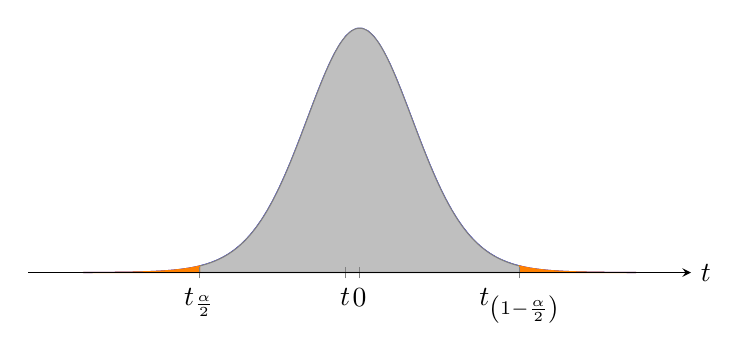
\begin{tikzpicture}[
        declare function={gamma(\z)=
          2.506628274631*sqrt(1/\z)+ 0.20888568*(1/\z)^(1.5)+ 0.00870357*(1/\z)^(2.5)- (174.2106599*(1/\z)^(3.5))/25920- (715.6423511*(1/\z)^(4.5))/1244160)*exp((-ln(1/\z)-1)*\z;},
        declare function={student(\x,\n)= gamma((\n+1)/2.)/(sqrt(\n*pi) *gamma(\n/2.)) *((1+(\x*\x)/\n)^(-(\n+1)/2.));}
        ]
    \begin{axis}[no markers, domain=-5:5, samples=100,
      axis x line=center,
      axis y line=none,
      xlabel=$t$, ylabel=$f_X(x)$,
      height=3cm, width=10cm,
      xtick={-2.8982, -.261, 0, 2.8982},
      xticklabels={$t_{\fr\alpha2}$,$t$, $0$,$t_{\lt(1-\fr\alpha2\rt)}$},
      ymax=.15,
      ytick=\empty,
      x label style={anchor=west},
      y label style={anchor=south},
      enlargelimits=true, clip=false, axis on top
      %grid style={line width=.1pt, draw=gray},
      % yticklabel style={
      %   /pgf/number format/fixed,
      %   /pgf/number format/fixed zerofill,
      %   /pgf/number format/precision=2
      % },        
      %   grid = major
      ]
      \addplot [blue, domain=-5:5] {student(x,17)};
      \addplot [gray, fill=gray!50, domain=-2.8982:2.8982] {student(x,17)} \closedcycle;
      \addplot [orange,fill=orange,  domain=-5:-2.8982] {student(x,17)} \closedcycle;
      \addplot [orange,fill=orange,  domain=2.8982:5] {student(x,17)} \closedcycle;
      % \node (d) at (axis cs: 6,.1) {Area: $1-\alpha$};
      %\draw[thick, ->] (d) -- (axis cs: .6,.05);
      %\node (c) at (axis cs: -8.5,.05) {Area: $\alpha$};
      %\draw[thick,->] (c) -- (axis cs: -6.5, 0.003);
    \end{axis}
  \end{tikzpicture}

\item We that the test statistic is within the region of nonrejection: \pause 
  \begin{equation*}
   t_{\fr\alpha2} = -2.8982 <  t = -0.261 < t_{\lt(1 - \fr\alpha2\rt)} = 2.8982
  \end{equation*}
    \end{enumerate}
  \end{exampleblock}
\end{frame}

\begin{frame}
  \begin{exampleblock}{Example 2: Golf ball production }
    \begin{enumerate}[Step 1.]\setcounter{enumi}{5}
    \item Thus, we \textbf{fail to reject} the null hypothesis. \\ \pause
      In real terms, this means that the sample was within the bounds of what would be acceptable if the population mean were 1.615 oz. Therefore, we would not stop the production line.
    \end{enumerate}
  \end{exampleblock}
\end{frame}

\section{$p$-values}

\begin{frame}
  \frametitle{Definition and usefulness of $p$-value}\pause
    \begin{block}{Definition}
    The $p$-value is the smallest level of significance at which $H_0$ would be rejected when a specified test procedure is used on a given dataset.
    \pause

    Equivalently, \pause this is the minimum probability of a Type I error.
  \end{block}
  
  \begin{itemize}[<+->]
  \item Provides more information about the strength of a test
  \item Indicates the smallest level at which the data is significant
  \item Can be compared with $\alpha$ irrespective of which type of test was used
  \end{itemize}
  \pause

  \begin{block}{Alternative definition}\pause
    The $p$-value is the probability of obtaining a test statistic value at least as contradictory to $H_0$ as the value that actually resulted.\pause

    \alert{The smaller the $p$-value, the more contradictory is the data to $H_0$.}
  \end{block}
\end{frame}


\begin{frame}
  \frametitle{$p$-value for $z$ tests}\pause

  \begin{minipage}{.6\linewidth}
  \begin{tikzpicture}[scale=.7]
    \begin{axis}[no markers, domain=0:10, samples=100,
      axis x line=center,
      axis y line=none,
      xlabel=$T$, ylabel=$f_X(x)$,,
      height=4cm, width=10cm,
      xtick={0,6},
      xticklabels={$0$,$t$},
      ymax=.15,
      ytick=\empty,
      x label style={anchor=west},
      y label style={anchor=south},
      enlargelimits=true, clip=false, axis on top
      %grid style={line width=.1pt, draw=gray},
      % yticklabel style={
      %   /pgf/number format/fixed,
      %   /pgf/number format/fixed zerofill,
      %   /pgf/number format/precision=2
      % },        
      %   grid = major
      ]
      \addplot [blue, domain=-10:10] {gauss(0,3)};
      \addplot [gray, fill=gray!50, domain=-10:6] {gauss(0,3)} \closedcycle;
      \addplot [orange,fill=orange,  domain=6:10] {gauss(0,3)} \closedcycle;
      \node (c) at (axis cs: 8.5,.05) {Area: $p$-value};
      \draw[thick,->] (c) -- (axis cs: 6.5, 0.003);
      % \draw[thick, |->] (axis cs: 6,-0.025) -- (axis cs: 10,-0.025) node[below,pos=.5] {\small\og Reject $H_0$};
    \end{axis}
  \end{tikzpicture}
\end{minipage}
\begin{minipage}{.35\linewidth}
  \begin{block}{$p$-value: area in upper tail}\pause
  \begin{equation}
    p  = 1 - F_T(t_\nu)\label{eq:41}
  \end{equation}
\end{block}

\end{minipage}

\pause

\bigskip

\begin{minipage}{.6\linewidth}
  \begin{tikzpicture}[scale=.7]
    \begin{axis}[no markers, domain=0:10, samples=100,
      axis x line=center,
      axis y line=none,
      xlabel=$T$, ylabel=$f_X(x)$,,
      height=4cm, width=10cm,
      xtick={-6,0},
      xticklabels={$t$,$0$},
      ymax=.15,
      ytick=\empty,
      x label style={anchor=west},
      y label style={anchor=south},
      enlargelimits=true, clip=false, axis on top
      ]
      \addplot [blue, domain=-10:10] {gauss(0,3)};
      \addplot [gray, fill=gray!50, domain=-6:10] {gauss(0,3)} \closedcycle;
      \addplot [orange,fill=orange,  domain=-10:-6] {gauss(0,3)} \closedcycle;
      %\node (d) at (axis cs: 6,.1) {Area: $1-\alpha$};
      %\draw[thick, ->] (d) -- (axis cs: .6,.05);
      \node (c) at (axis cs: -8.5,.05) {Area: $p$-value};
      \draw[thick,->] (c) -- (axis cs: -6.5, 0.003);
    \end{axis}
  \end{tikzpicture}
\end{minipage}
\begin{minipage}{.35\linewidth}
  \begin{block}{$p$-value: area in lower tail} \pause
    \begin{equation}
    p  = F_T(t_\nu) \label{eq:42}
  \end{equation}
\end{block}

  
\end{minipage}

\pause
\bigskip

\begin{minipage}{.6\linewidth}
  \begin{tikzpicture}[scale=0.7]
    \begin{axis}[no markers, domain=0:10, samples=100,
      axis x line=center,
      axis y line=none,
      xlabel=$T$, ylabel=$f_X(x)$,,
      height=4cm, width=10cm,
      xtick={-6,0,6},
      xticklabels={$-t$,$0$,$t$},
      ymax=.15,
      ytick=\empty,
      x label style={anchor=west},
      y label style={anchor=south},
      enlargelimits=true, clip=false, axis on top
      %grid style={line width=.1pt, draw=gray},
      % yticklabel style={
      %   /pgf/number format/fixed,
      %   /pgf/number format/fixed zerofill,
      %   /pgf/number format/precision=2
      % },        
      %   grid = major
      ]
      \addplot [blue, domain=-10:10] {gauss(0,3)};
      \addplot [gray, fill=gray!50, domain=-6:6] {gauss(0,3)} \closedcycle;
      \addplot [orange,fill=orange,  domain=6:10] {gauss(0,3)} \closedcycle;
      \addplot [orange,fill=orange,  domain=-10:-6] {gauss(0,3)} \closedcycle;
      \node (c) at (axis cs: 8.5,.05) {Area: $0.5p$-value};
      \draw[thick,->] (c) -- (axis cs: 6.5, 0.003);
      \node (e) at (axis cs: -8.5,.05) {Area: $0.5p$-value};
      \draw[thick,->] (e) -- (axis cs: -6.5, 0.003);
    \end{axis}
  \end{tikzpicture}
\end{minipage}
\begin{minipage}{.35\linewidth}
  \begin{block}{$p$-value: sum of area in both tails} \pause
  \begin{equation}
    \label{eq:43}
    p = 2 (1 - F_T|t_\nu|))
  \end{equation}
\end{block}

\end{minipage}
\end{frame}

%\end{comment}

\section{Inference on regression coefficient estimates}
\begin{frame}
  \frametitle{Estimates and standard error}
  From the model equation $Y = w_0 + w_1 X + \epsilon$, we see that $Y$ is a random variable with true variance $\sigma^2$.\\ \pause

  The point estimate of the true mean of $Y$ is unbiased: \pause

  \begin{align}
    \label{eq:10}
    \hat \mu       = \ol y &= \fr 1n \sum y_n\\
    \mb{E}(\hat \mu ) &= \mu
  \end{align}

  Based on the Gauss-Markov theorem, the least squares estimates are also unbiased: \pause

  \begin{align}
    \label{eq:11}
    E\lt(\hat w_0 \rt) = w_0 \\
    E\lt(\hat w_1 \rt) = w_1
  \end{align}
\end{frame}

\begin{frame}
  \frametitle{Standard errors}
  The population of $Y$ is unknown, but we can estimate its parameters from a sample of $n$ observations.\\ \pause

  \bigskip
  
  By the Central Limit Thereom (CLT), $\ol Y$ is normally distributed with mean $\mu$ and variance $\sigma^2/n$.\\ \pause

  \bigskip

  \begin{block}{Standard error}
    The standard error of mean estimate is given by:
    \begin{equation}
      \label{eq:12}
      S\mb{E}(\hat\mu) = Var(\hat\mu) = \fr{\sigma}{\sqrt{n}}
    \end{equation}
  \end{block}

  Where $\sigma$ is not known, it can be estimated from the data:\pause
  \begin{equation}
    \label{eq:12a}
    \hat\sigma^2 = \pause \fr{\sum \lt(y - \hat y\rt)^2}{N-2} = \pause \fr{RSS}{N-2} = RSE^2
  \end{equation}
\end{frame}
\begin{frame}
  \frametitle{Model accuracy}\pause

  We use the standard errors to evaluate the accuracy of the coefficient estimates.\pause
  
  \begin{align}
    \label{eq:3}
    Var(\hat\mu) &= SE(\hat\mu)^2 = \fr{\sigma^2}{n}\\ \pause
    SE(\hat w_0)^2     &= \sigma^2\lt[\fr1n + \fr{\ol x^2}{\sum_{i=1}^N(x_n - \ol x)^2}\rt] \\ \pause
    SE(\hat w_1)^2     &= \fr{\sigma^2}{\sum_{i=1}^N(x_n - \ol x)^2}
  \end{align}
  \pause

  
\end{frame}

\begin{frame}
  \frametitle{Hypothesis testing on the slope parameter}
  \pause

  The so-called \textbf{\rd model utility test} is used to determine if any relationship exists between $X$ and $Y$.\pause

  \bigskip

  \textbf{Null hypothesis:}
  \pause
  \begin{equation}
    \label{eq:13}
    H_0 : w_1 = 0 
  \end{equation}
  \pause

  \textbf{Alternative hypothesis:}\pause
  \begin{equation}
    \label{eq:14}
    H_1 : w_1 \ne 0
  \end{equation}

  \pause

  \textbf{Test statistic:}\pause
  \begin{equation}
    \label{eq:15}
    t = \fr{\hat w_1}{SE\lt(\hat w_1\rt)}
  \end{equation}
  \pause

  \begin{alertblock}{Decision}\pause
    Reject null hypothesis  if $t\le t_{\alpha/2,N-2}$  or $t \ge t_{1-\alpha/2,N-2}$.
  \end{alertblock}
\end{frame}

\begin{frame}
  \frametitle{Regression and the $F$ test }\pause

  The right-tail $F$ test gives the exact same result as the model utility $t$ test because: \pause

  \begin{itemize}[<+->]
  \item $t^2 = f$
  \item $t^2_{1 - \alpha/2, N-2} = F_{1 -\alpha, 1, N-2}$ (critical value)
  \end{itemize}

  \pause

  \bigskip
  
  Analysis of variance (ANOVA) table for simple linear regression:

  \pause
  
  \begin{tabular}{l c c c c}\toprule
    \bf Source of  & \bf d.o.f. & \bf Sum of  & \bf Mean         & $\bm F$   \\ 
    \bf variation  &            & \bf Squares   &       \bf Square   &           \\ \midrule \pause
    Regression              & 1          & $TSS-RSS$              & $TSS-RSS$                  & $\fr{(TSS-RSS)}{RSS/(N-2)}$ \\ \pause
    Error                   & $N-2$      & $RSS$              & $RSE^2 = \fr{RSS}{N-2}$  &  \\  \midrule  \pause
    Total                   & $N-1$      & $TSS$              &                        &  \\ \bottomrule
  \end{tabular}
\end{frame}


\begin{frame}
  \frametitle{Confidence intervals}
  The $100(1-\alpha)\%$ confidence intervals of the coefficient estimates are given by: \pause
  \begin{align}
    \label{eq:18}
    \langle w_0\rangle_{1-\alpha} &= \hat w_0 \pm t_{\lt(1 -\fr\alpha2, N-2\rt)} SE\lt(\hat w_0\rt)\\[2mm]
    \langle w_1\rangle_{1-\alpha} &= \hat w_1 \pm t_{\lt(1 -\fr\alpha2, N-2\rt)} SE\lt(\hat w_1\rt)
  \end{align}
\end{frame}



 



\begin{frame}
  \frametitle{$R^2$ and correlation coefficient}
  \pause

  Recall the \textbf{sample correlation coefficient}: \pause

  \begin{equation}
    \label{eq:19}
    r = \fr{\sum(x_n - \ol x)(y_n - \ol y)}{\sqrt{ \sum(x_n - \ol x)^2 \sum(y_n - \ol y)^2}}
  \end{equation}

  \pause

  In the univariate case, we can show that $R^2 = r^2$.\\ \pause

  \bigskip
  
  Thus, $R^2$ is also a measure of the linear relationship between $X$ and $Y$.

  
\end{frame}
 

\end{document}

%%% Local Variables:
%%% mode: latex
%%% TeX-master: t
%%% End:
